% General settings
\documentclass[slidestop,compress,9pt]{beamer}
\usetheme{AnnArbor}
\usepackage[UKenglish]{babel}
\usepackage[UKenglish]{isodate}
\usepackage[utf8]{inputenc}
\usepackage{hyperref}
\definecolor{links}{HTML}{2A1B81}
\hypersetup{colorlinks=true,allcolors=links}

% Code listings and pseudocode
\usepackage{listings}
\usepackage{algpseudocode}
\usepackage{algorithm}

% Mathematical formulas
\usepackage{mathtools}
\usepackage{bm}
\setcounter{MaxMatrixCols}{20}

% Graphics and figures
\usepackage{graphicx}
\graphicspath{{figures/}}
\setbeamertemplate{caption}[numbered]
\usepackage{fancybox}
\usepackage{pgfplots}

% Tikz
\usepackage{tikz}
\usepackage{tikz-3dplot}
\usetikzlibrary{shapes.geometric, arrows}

% For redefinition of texttt
%\let\textttorig\texttt
\usepackage[scaled=1.0]{couriers}

\setbeamertemplate{frametitle}{\insertsection\hspace*{0.45cm}\insertframetitle}

% Numbered sections
\setbeamertemplate{section in toc}[sections numbered]
\setbeamertemplate{subsection in toc}[subsections numbered]
\setbeamertemplate{subsubsection in toc}[subsubsections numbered]

% Listings
\definecolor{cident}{rgb}{0.0,0.0,0.0}
\definecolor{ckeyw}{rgb}{0,0,0.8}
\definecolor{ccomm}{rgb}{0,0.8,0}
\definecolor{cstr}{rgb}{0.8,0,0}
\definecolor{myyellow}{rgb}{0.99,0.76, 0.0}
\definecolor{mymagenta}{rgb}{1.0, 0.0, 1.0}

\lstset{language=[LaTeX]{TeX},
  basicstyle=\normalsize\ttfamily,
  keywordstyle=\color{ckeyw}\bfseries,
  identifierstyle=\color{cident}\bfseries,
  commentstyle=\color{ccomm},
  stringstyle=\color{cstr},
  showstringspaces=false,
  breaklines=true,
  breakatwhitespace=true,
  tabsize=2,
  mathescape = false,
  columns=flexible,
  escapeinside={<@}{@>}
%   numbers=left,
%   stepnumber=1,
%   firstnumber=1,
%   numberfirstline=true,
  }

\title[The oxDNA Coarse-Grained Model of DNA and RNA]{\textbf{The oxDNA Coarse-Grained Model of DNA}}
\subtitle{An Introduction to the Model and Software Framework }
\author[Oliver Henrich]{Oliver Henrich \\ \small Email: \href{mailto:oliver.henrich@strath.ac.uk}{oliver.henrich@strath.ac.uk}}
\institute[U Strathclyde, Glasgow, UK]{Department of Physics, University of Strathclyde, Glasgow, UK}
\date{22nd September 2022}


\begin{document}

%\renewcommand<>{\texttt}[1]{%
%  \only#2{\textttorig{#1}}%
%}

\renewcommand<>{\texttt}{\only#1{\beameroriginal{\texttt}}}

% ==============================================================
% --- Welcome frame
% ==============================================================
\begin{frame}[plain]
\maketitle
\end{frame}

% ==============================================================
% --- TOC
% ==============================================================

\begin{frame}
\Large Outline
\tableofcontents
\normalsize
\end{frame}

% ==============================================================
% --- Content
% ==============================================================

\section{oxDNA Model}

\begin{frame}
\frametitle{DNA Facts}

\begin{itemize}
\item Human genome contains $3\times10^{9}$ base pairs (bps)
\item DNA loop around a nucleosome core particle contains 147 bps
\item Smallest loop in chromatin fibre consists of $5\times10^4$ bps
\item Atomistic simulation of DNA can model 3,000 bps (probably less) and typically resolve times on the $\mu$s-scale  
\item Coarse-grained models target much larger time and length scales in the range of ms and Mbps 
\end{itemize}

\begin{center}
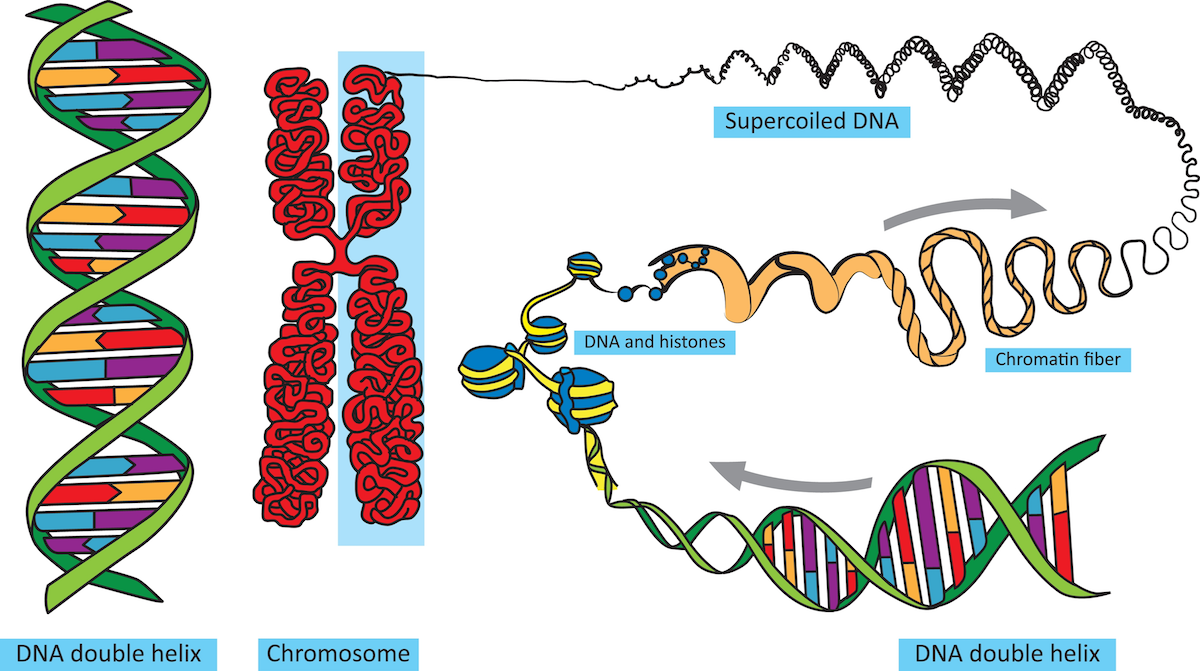
\includegraphics[width=0.54\textwidth]{fromDNAtoChromatin.png}
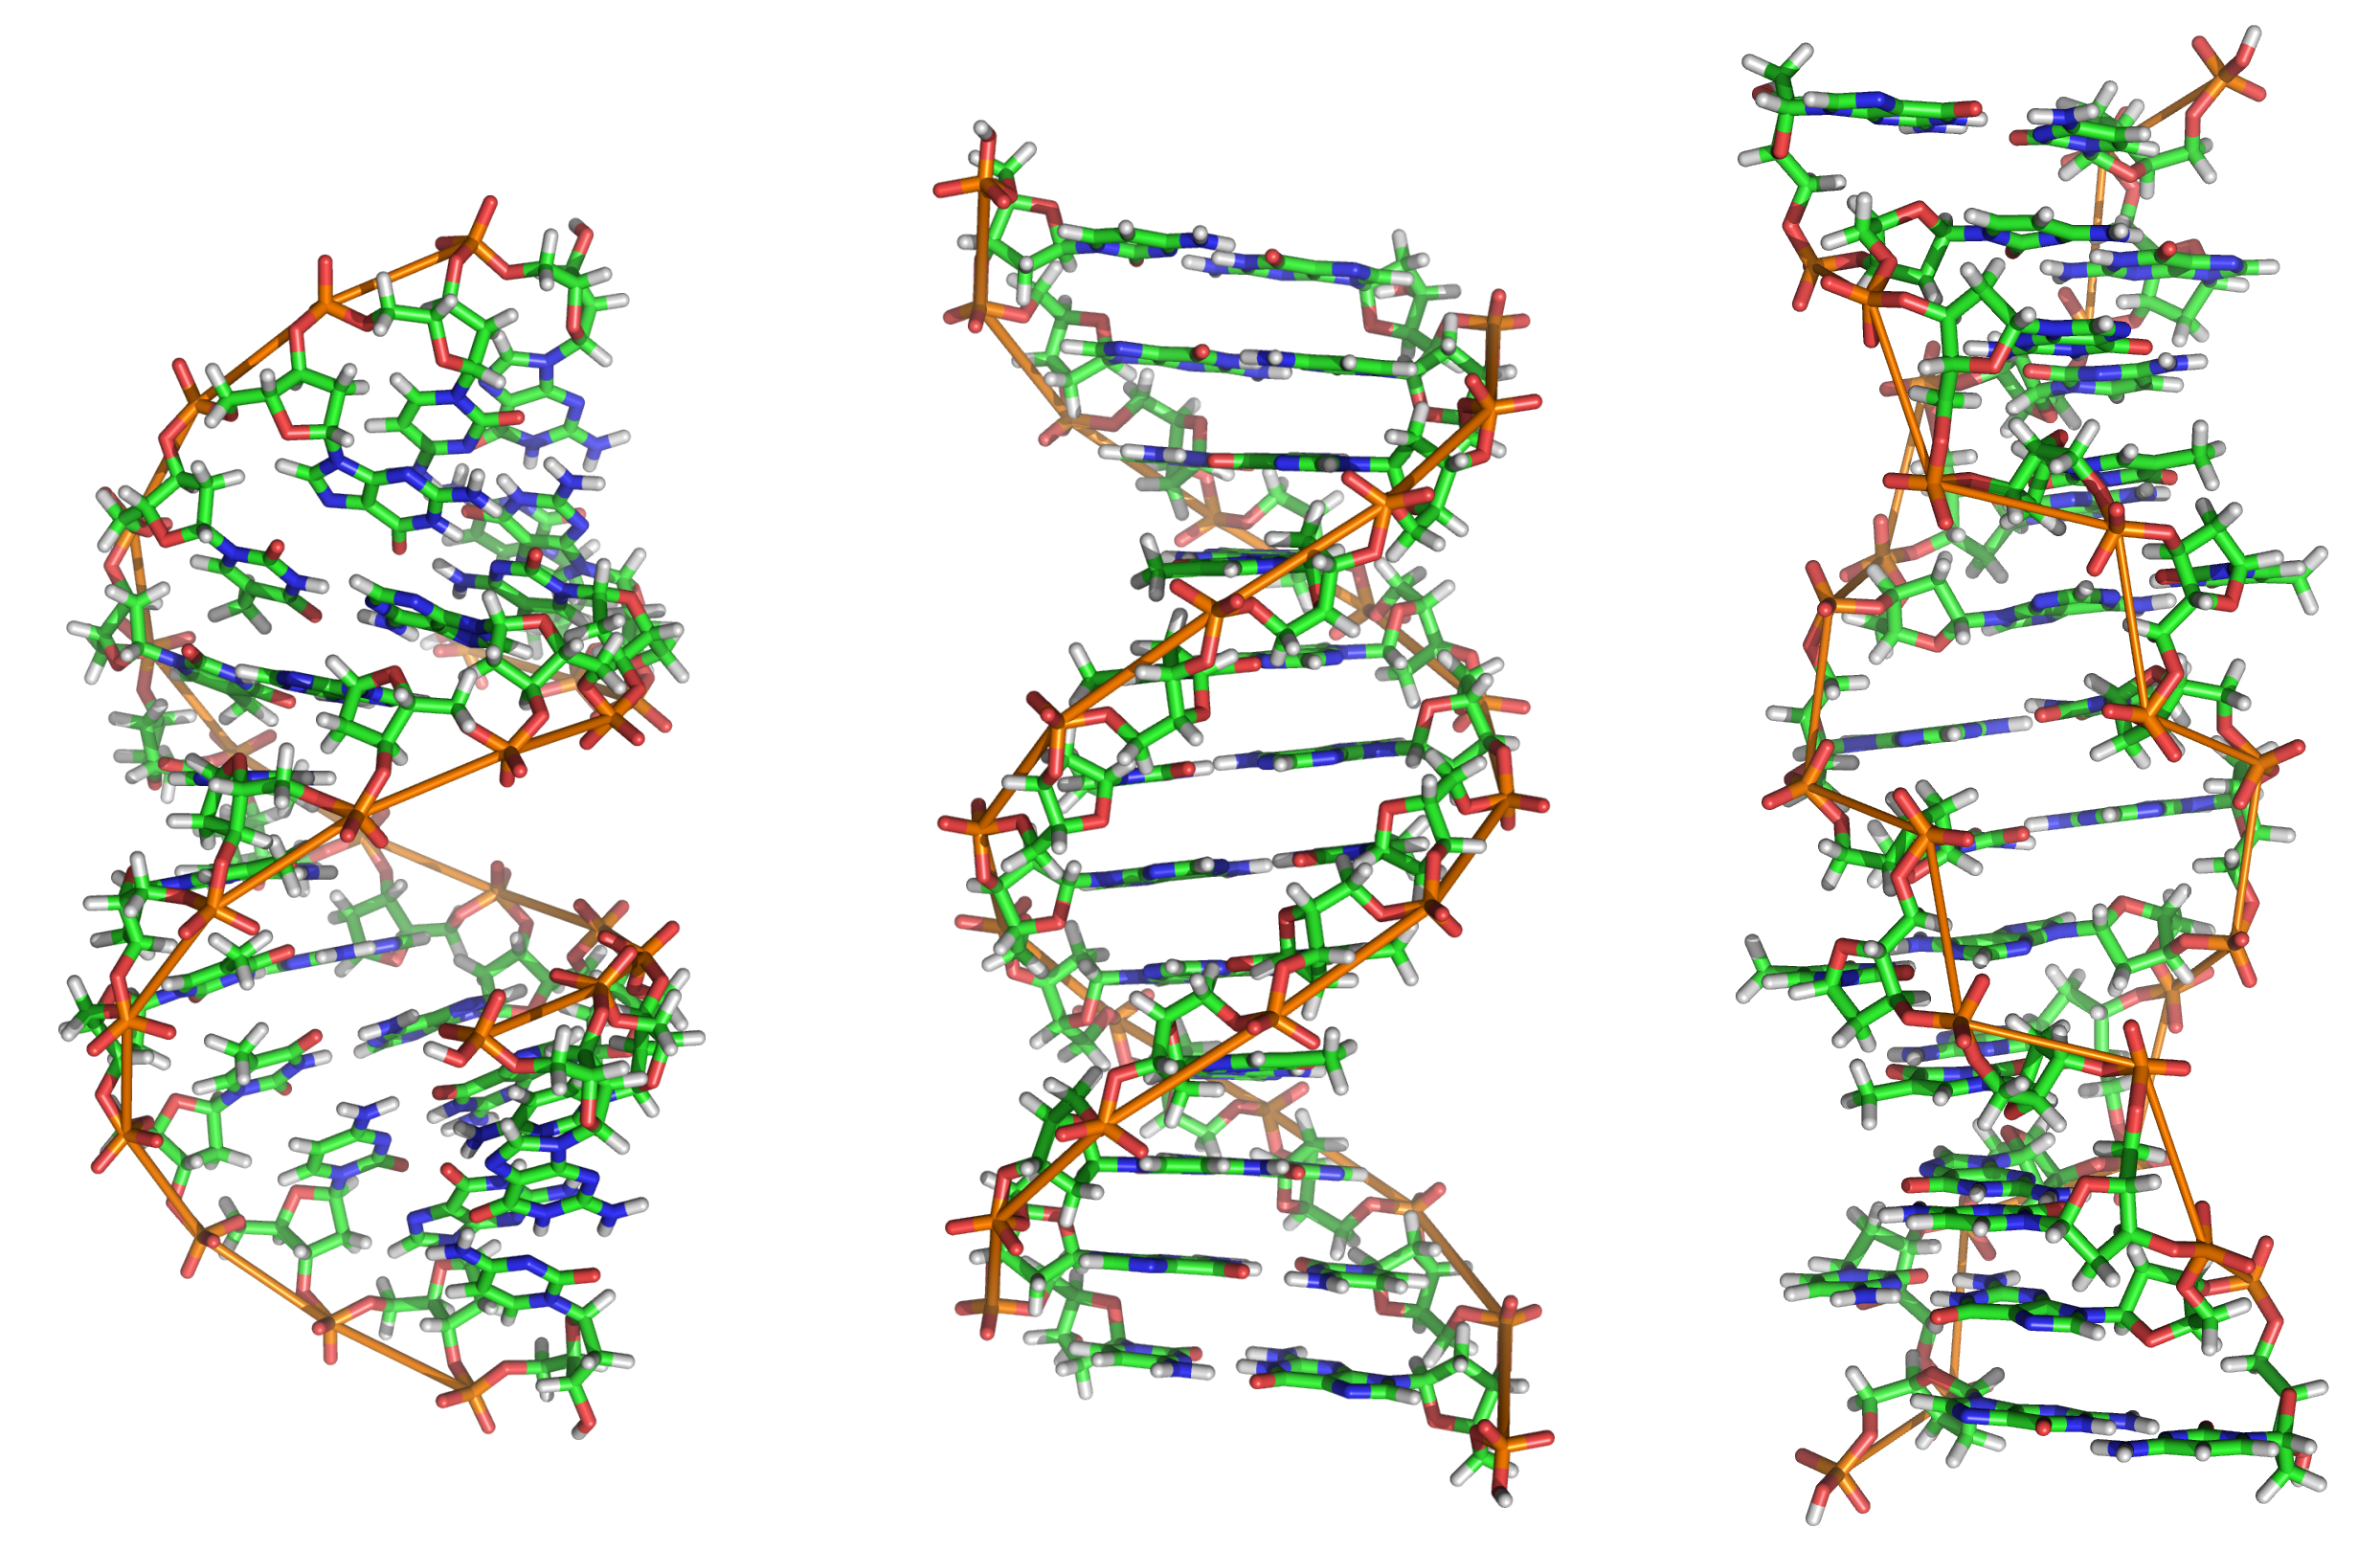
\includegraphics[width=0.45\textwidth]{A-B-Z-DNA.png}\\
From DNA to chromatin \hspace{2.75cm} A-DNA, B-DNA, Z-DNA
\end{center}

\end{frame}

\begin{frame}
\frametitle{Overview}

\begin{itemize}
\item Each nucleotide is described as rigid body
\item 3 interaction sites for backbone, stacking and hydrogen-bonding
\item 7 effective interactions between nucleotides
\begin{itemize}
\item Bonded interaction for backbone connectivity
\item 6 pair interactions for excluded volume, stacking, cross-stacking, coaxial stacking, hydrogen-bonding and electrostatic interaction
\end{itemize}
\item oxDNA: 13 DOF per nucleotide\\
3 positions, 3 translational momenta, 3 angular momenta, 1 unit quaternion (4 components)
\item Atomistic simulation (e.g. thymine): around 200 DOF per nucleotide\\
34 atoms per nucleotide, each with 3 positions and 3 momenta
\end{itemize}

\vspace*{-0.5cm}

\begin{columns}
\begin{column}{0.4\textwidth}
\begin{center}
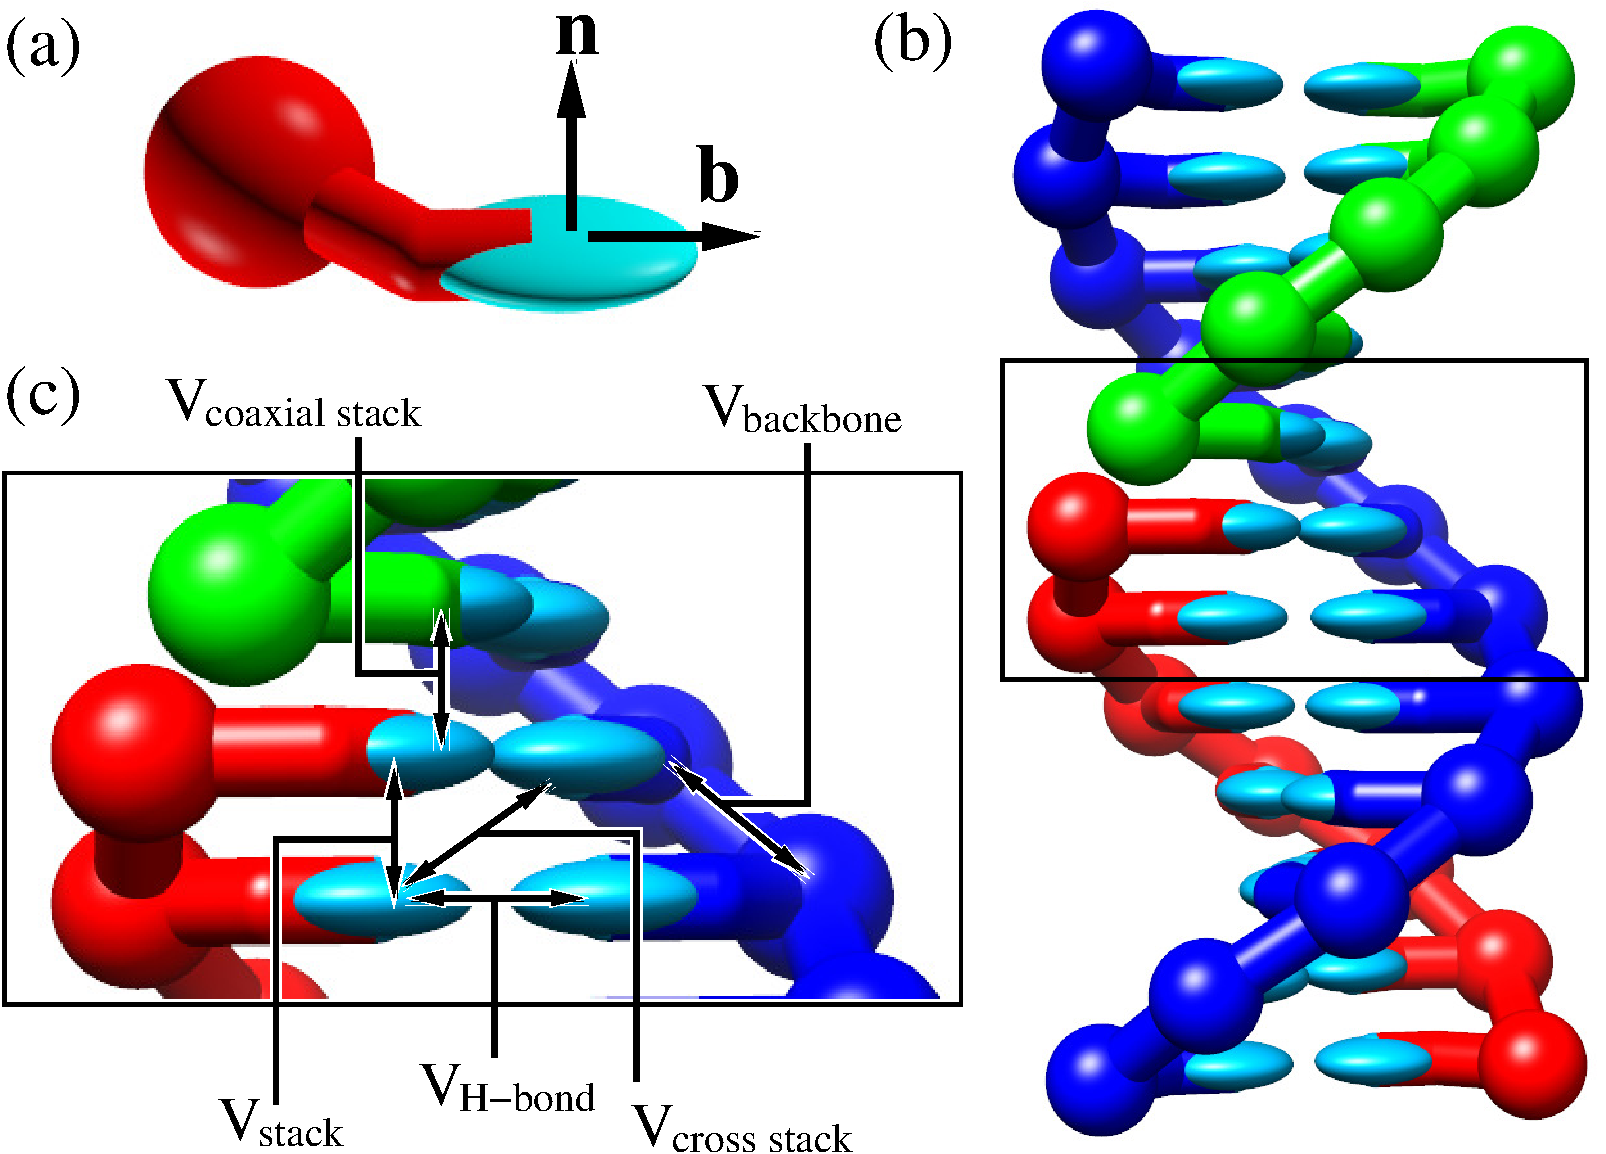
\includegraphics[width=0.9\textwidth]{nucleotide_duplex_b.pdf}
\end{center}
\end{column}

\begin{column}{0.45\textwidth}
\begin{center}
\vspace*{0.5cm}
\begin{itemize}
\setlength\itemsep{7pt}
\item[] (a) oxDNA nucleotide
\item[] (b) Duplex
\item[] (c) Interactions
\end{itemize}
\end{center}
\end{column}
\end{columns}

\end{frame}

\begin{frame}
\frametitle{Nucleotide Geometry}

\begin{columns}
\begin{column}{0.46\textwidth}
\begin{itemize}
\setlength\itemsep{7pt}
\item Each nucleotide has a centre of mass (COM) $\bm{r}_{COM}$, a base vector $\bm{b}$, base normal $\bm{n}$ and a third vector $\bm{y}=\bm{n}\times\bm{b}$
\item The \textbf{backbone interaction} site is at\\
$\bm{r}_{COM} - 0.4\,\bm{b}$ \hspace{1.7cm}(oxDNA1)\\
$\bm{r}_{COM} - 0.34\, \bm{b} + 0.3408\,\bm{y}$ (oxDNA2)
\item The \textbf{stacking interaction} site is at\\
$\bm{r}_{COM} + 0.34\, \bm{b}$
\item The \textbf{hydrogen-bonding interaction} site is at\\
$\bm{r}_{COM} + 0.4\, \bm{b}$
\end{itemize}
\end{column}

\begin{column}{0.54\textwidth}
\vspace*{-0.5cm}
\begin{center}
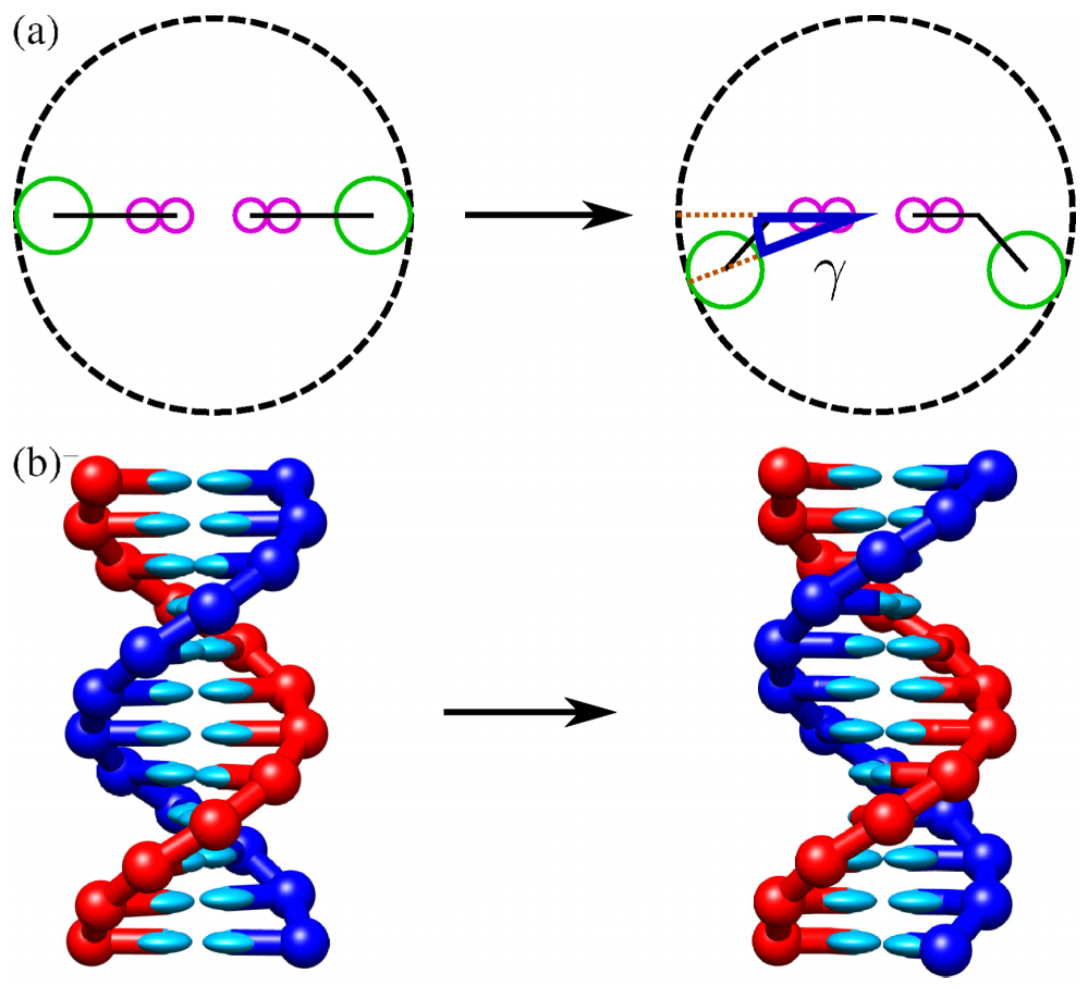
\includegraphics[width=0.8\textwidth]{oxdna_oxdna2.png}\\
\end{center}
(a) oxDNA1 and oxDNA2 nucleotides: the base vector is horizontally oriented from left to right, whereas the base normal points away from the observer.\\
(b) The angled backbone interaction sites leads to the correct geometry with major and minor grooves. 
\end{column}
\end{columns}

\end{frame}

\begin{frame}
\frametitle{Interactions}

\begin{columns}
\begin{column}{0.49\textwidth}

\end{column}

\begin{column}{0.45\textwidth}
\begin{center}
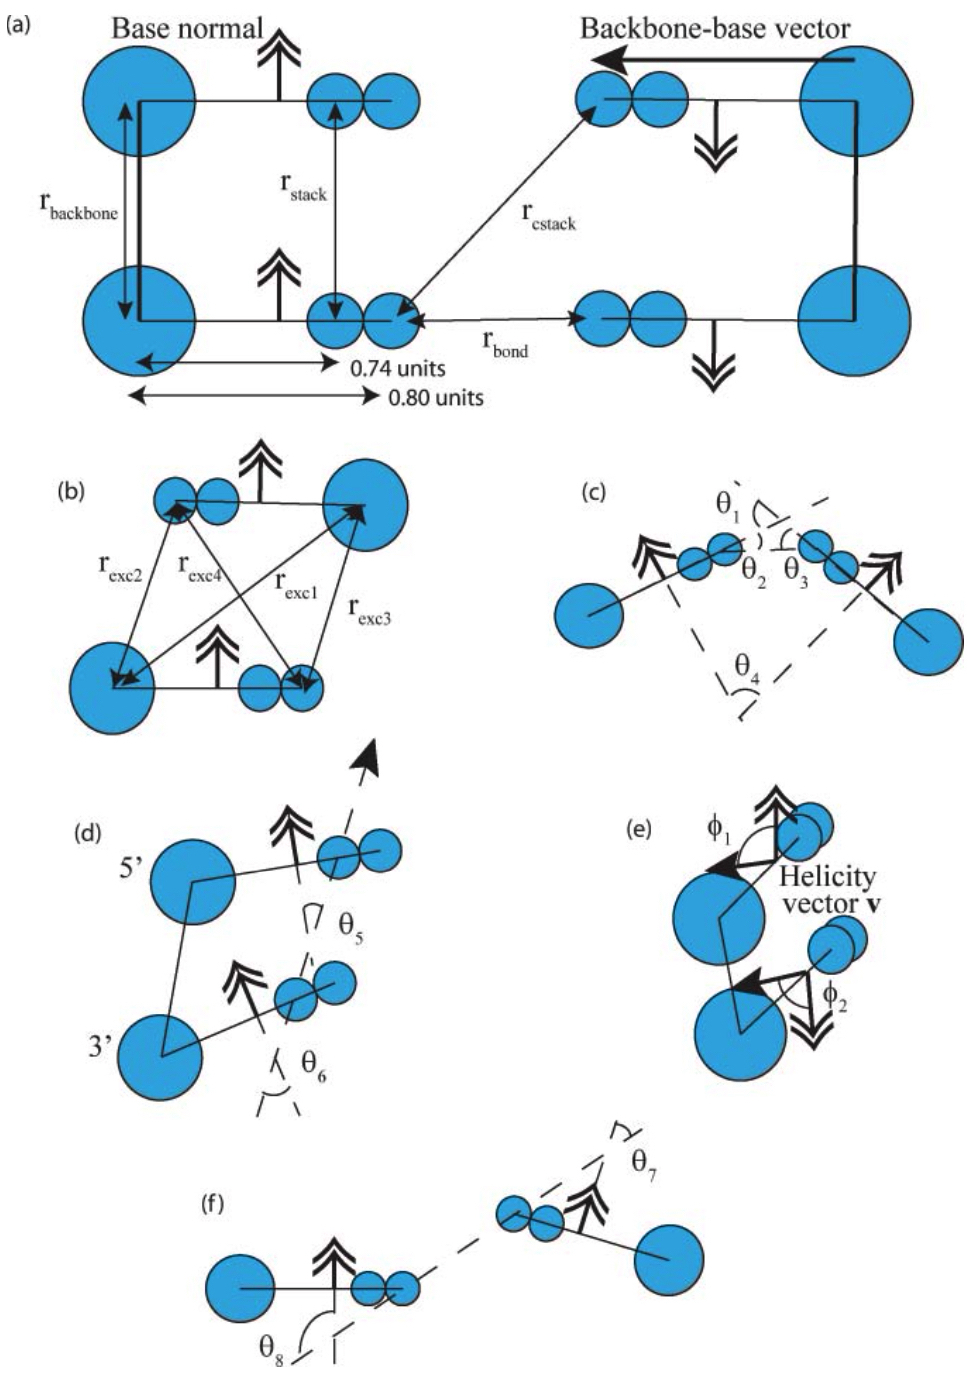
\includegraphics[width=0.9\textwidth]{oxdna.jpg}
\end{center}
\end{column}
\end{columns}

\end{frame}

\begin{frame}
\frametitle{}

\end{frame}


\section{oxDNA Software}

\begin{frame}
\frametitle{LAMMPS version}
BlaBla

\end{frame}

\begin{frame}
\frametitle{Standalone version}
BlaBlaBla

\end{frame}

\section{Practical}

\begin{frame}
\frametitle{Melting}
BlaBlaBlaBlub

\end{frame}

\end{document}
